\documentclass[11pt, oneside]{article}   	% use "amsart" instead of "article" for AMSLaTeX format
\usepackage{geometry}                		% See geometry.pdf to learn the layout options. There are lots.
\geometry{letterpaper}                   		% ... or a4paper or a5paper or ... 
%\geometry{landscape}                		% Activate for for rotated page geometry
%\usepackage[parfill]{parskip}    		% Activate to begin paragraphs with an empty line rather than an indent
\usepackage{graphicx}				% Use pdf, png, jpg, or eps� with pdflatex; use eps in DVI mode
								% TeX will automatically convert eps --> pdf in pdflatex		
\usepackage{amssymb}
\usepackage{amsmath}

\title{Cone and Sphere by Disks and Shells}
%\author{The Author}
\date{}							% Activate to display a given date or no date

\graphicspath{{/Users/telliott_admin/Dropbox/Tex/png/}}

\begin{document}

\maketitle
%\section{}
% \subsection*{R code}
% \begin{lstlisting}  \end{lstlisting}
% \begin{center} 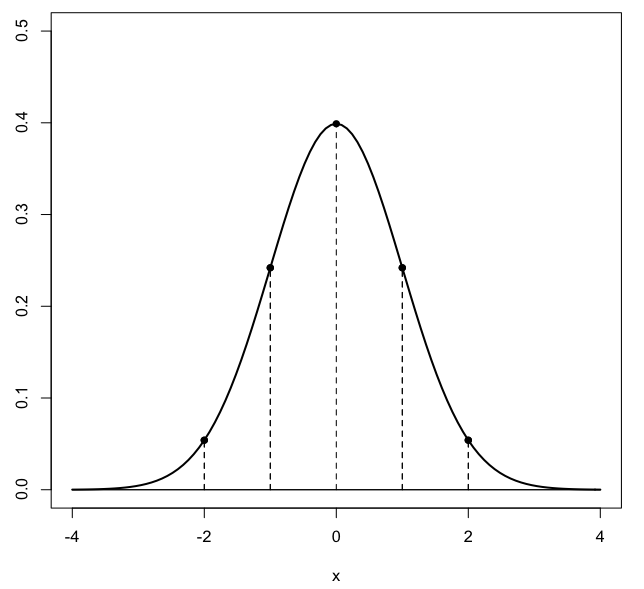
\includegraphics [scale=0.4] {gauss3.png} \end{center}
% \begin{bmatrix} a  &  b \\ c  &  d \end{bmatrix}
% \bigg |_

\Large
\noindent

\begin{center} 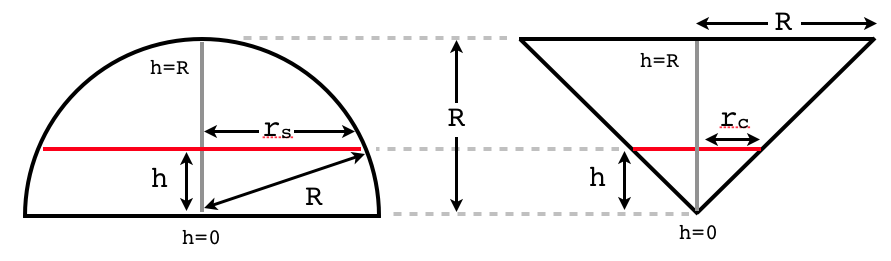
\includegraphics [scale=0.4] {sphere_cone.png} \end{center}
Here is a figure that I used previously in the write-up about Archimedes, who found a formula for the volume of a sphere by subtracting a cone (or two cones) from a cylinder.  The volume of a cone was previously known to be
\[ V_{cone} = \frac{1}{3} \pi R^2H, \ \ \text{for} \ H=R, \ \ V_{cone} = \frac{1}{3} \pi R^3 \]
for a cone with base radius $R$ and height $H$.  Any solid of this type has the formula $1/3$ base area $\times$ height.
\subsection*{Disks}
We can use calculus to derive this formula.  We think of slicing the volume horizontally into a series of disks.  If the height at any point is $h$, with total height $H$ and radius $R$, then by similar triangles the radius (right hand panel above) is
\[ r = h\frac{R}{H} \]
the area of each disk is
\[ A = \pi r^2 = \pi \frac{R^2}{H^2} h^2 \]
and what we need to do is to add up all the disks for $h=0 \to h=H$
\[ V = \int A \ dh = \int_{h=0}^{h=H} \pi \frac{R^2}{H^2} h^2 \ dh \]
\[ = \frac{1}{3}\pi \frac{R^2}{H^2}\ h^3 \bigg|_0^H = \frac{1}{3}\pi R^2 H \]
\begin{equation}
\boxed{V = \frac{1}{3}\pi R^2 H}
\end{equation}

\subsection*{Shells}
There is another way to "slice" the figure, which is called the method of shells.
\begin{center} 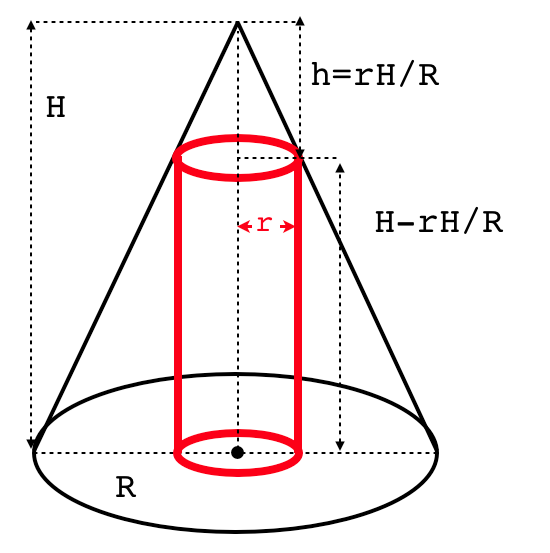
\includegraphics [scale=0.4] {cone_shell2.png} \end{center}
We think of the volume as constructed from a series of concentric cylinders.  Let's use the same letters we had previously, $H$ for total height and $R$ for base radius.  At a height $h$ measured down from the top, the radius $r$ is, as before
\[ r = h\frac{R}{H} \]
We have a cylinder whose circumference is
\[ C = 2\pi r = 2\pi h\frac{R}{H} \]
The height of the cylinder is $H-h$, and the lateral surface area of the shell is
\[ SA = C(H-h) = 2\pi h\frac{R}{H}(H-h) = 2\pi \frac{R}{H} (Hh-h^2)\]
We add up all the shells for $h=0 \to h=H$
\[ V = \int A \ dh = \int_0^H 2\pi \frac{R}{H} (Hh-h^2) \]
\[ = 2\pi \frac{R}{H}(\frac{1}{2}Hh^2 - \frac{1}{3}h^3) \bigg|_0^H = 2\pi \frac{R}{H}(\frac{1}{6}H^3 ) = \frac{1}{3} \pi R^2H \] 
\subsection*{Varying $r$ instead of $h$}
\begin{center} 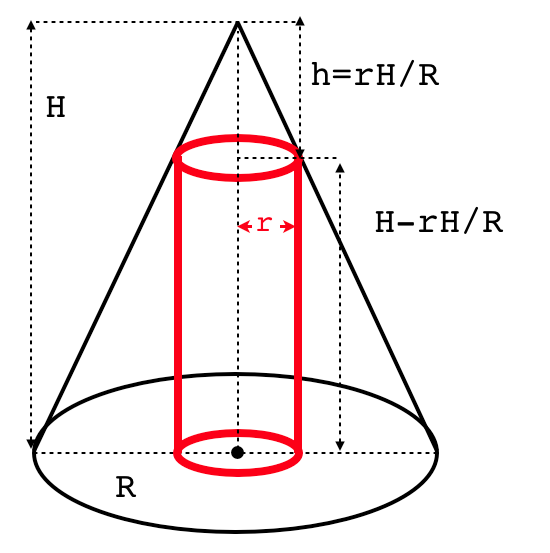
\includegraphics [scale=0.4] {cone_shell2.png} \end{center}
In the previous section we used $h$ as the variable of integration, but we might just as well have used $r$.  In that case, $r$ will vary from $r=0 \to r=R$.  At each value, the circumference will be
\[ C = 2 \pi r \]
and the height of the cylinder will be
\[ H-\frac{H}{R}r \]
The volume is the sum of all the little pieces of cylinder volume
\[ V = \int_{r=0}^{r=R} 2 \pi r (H -\frac{H}{R}r) \ dr \]
\[ = 2 \pi H \int_{r=0}^{r=R} r  - \frac{1}{R}r^2 \ dr = 2 \pi H \ (\frac{r^2}{2} - \frac{1}{R}\frac{r^3}{3}) \  \bigg|_0^R = 2 \pi H (\frac{1}{6} R^2) = \frac{1}{3} \pi R^2H \]
\subsection*{Lateral surface area}
We can use a similar method for the surface area (not counting the base).  We go back to the picture with slices.  Each slice has a circumference of $2 \pi r$.

If we look at the slices, the height of each is $dh$, but the actual length of the area element is elongated because of the slanted side.  If we call the angle between the slanted side and the horizontal $\theta$, and the length of the slanted side is $S$
\[ \frac{H}{S} = sin \ \theta \]
\[ H = S \ sin \ \theta \]
\[ dh = ds \ sin \ \theta \]
so the element of surface area is $dA = C \ ds$.  We add them all up
\[ SA = \int C \ ds = \int 2 \pi r \ ds \]
\[ = \int 2 \pi r \frac{1}{sin \ \theta} \ dh = \frac{2\pi}{sin \ \theta} \int r \  dh\]
Now substitute for $r$
\[= \frac{2\pi}{sin \ \theta}  \int_{h=0}^{h=H} \frac{R}{H} h \ dh \]
\[ = \frac{2\pi}{sin \ \theta} \frac{R}{H} \ [\frac{h^2}{2} ] \bigg|_0^H \]
\[ = \frac{\pi}{sin \ \theta} R H  \]
\begin{equation}
\boxed{SA = \pi RS}
\end{equation}

\subsection*{Volume of the sphere by disks}
\begin{center} 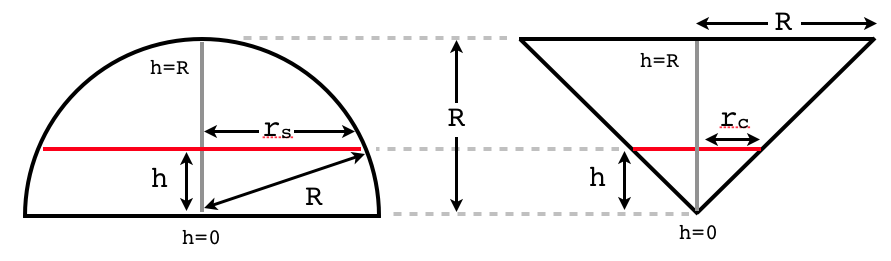
\includegraphics [scale=0.4] {sphere_cone.png} \end{center}
Going back to the figure with the hemisphere in it, we will slice this into horizontal disks of radius $r$.  If we label the height $h$ as shown in the figure, increasing from $0$ at the bottom to  $h=R$ at the top, then for the slice at each position $h$ we have a circle with area 
\[ A = \pi r^2 = \pi (R^2-h^2)  \]
The little bit of volume is
\[ dV = A \ dh =  \pi (R^2-h^2) \ dh \]
We integrate (add up all these slices)
\[ \int_{h=0}^{h=R} \pi (R^2-h^2) \ dh = \pi \ [ \ R^2h - \frac{h^3}{3}\ ] \ \bigg|_0^R = \frac{2}{3} \pi R^3 \]
Since this is for the hemisphere, the sphere is twice the value or $(4/3) \pi R^3$, as expected.

\subsection*{Volume of the sphere by shells}
For all of these examples, we can let either $r$ or $h$ be the variable of integration, since there is a simple relationship between $r$ and $h$.  For the cylinder it involves the ratio $R/H$, and for the sphere
\[ h^2 + r^2 = R^2 \]
when $h = 0$ at the "fat end" of the solid.  A different but still simple formula can be found when $h=0$ at the tip of the solid.

Let's divide the sphere up into concentric cylinders or shells, and let $r$ vary from $0 \to R$.  The circumference of the shell at each point is 
\[ C = 2 \pi r \]
and the height of each is 
\[ h = \sqrt{R^2 - r^2} \]
The volume of each very thin cylinder is
\[ dV = Ch \ dr = 2 \pi r \sqrt{R^2 - r^2} \ dr \]
and we want
\[ \int_{r=0}^{r=R} 2 \pi r \sqrt{R^2 - r^2} \ dr \]
\[ = -\frac{2}{3}\pi (R^2 - r^2)^{3/2} \bigg|_0^R = -\frac{2}{3}\pi \ [ \ - (R^2)^{3/2} \ ] = \frac{2}{3} \pi R^3 \]
as before.

Here is a picture of what we're doing, from Hamming's Calculus text.  The notation is different but the idea is the same.

\begin{center} 
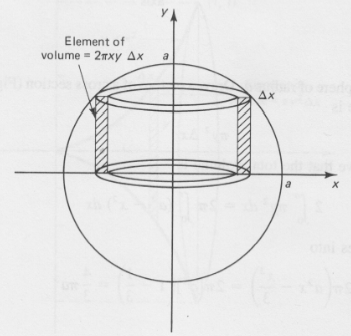
\includegraphics [scale=0.6] {sphere_vol2.png} 
\end{center}

\subsection*{Surface area of a sphere}
My favorite way of doing this is the simplest.  Suppose we have a sphere with radius $r$ and we increase $r$ by a little bit $dr$.  What is the change in volume, $dV$?  It's the surface area times $dr$
\[ dV = SA \ dr \]
\[ SA = \frac{dV}{dr} = \frac{d}{dr} \ (\frac{4}{3}\pi r^3) = 4 \pi r^2 \]
A bit fancier method is to imagine we revolve a function $y = f(x)$ around the x-axis.  To compute the surface area of the solid, we slice it into disks in the usual way, but moving along the x-axis in increments $dx$.  Then we need to find the surface area of the disk.  In this situation, the elements of surface area $ds$ are given by:
\[  ds = \sqrt{1 + (\frac{dy}{dx})^2} \ dx \]
After setting up $ds$, we will integrate
\[  \int 2 \pi y \ ds \]
If we have a circle with radius $R$ centered at the origin.
\[ x^2 + y^2 = R^2;  \ \  y = f(x) = \sqrt{R^2 - x^2} \]
Using implicit differentiation, it is easy to show that
\[ 2x \ dx + 2y \ dy = 0 \]
\[ \frac{dy}{dx} = -x/y \]
Then
\[ ds = \sqrt{1 + \frac{x^2}{y^2}} \ dx =  \sqrt{1 + \frac{x^2}{(R^2 - x^2)}} \ dx \]
And
\[ SA = 2 \pi \int y \ ds = 2 \pi \int   \sqrt{(R^2-x^2)} \  \sqrt{1 + \frac{x^2}{(R^2 - x^2)}} \ dx \]
\[ 2 \pi \int   \sqrt{R^2 - x^2 + x^2 } \ dx = 2 \pi \int R \  dx = 2 \pi R x \]
I do like the way that simplifies!.  Now evaluate from $x = -R \to R$, giving:
\[ SA = 4 \pi R^2 \]
The expected result.



\end{document}  